% LaTeX Tables for Brent Oil and Indian Oil Stocks Analysis
% Generated from analysis results (2014-2024)

\documentclass[11pt]{article}
\usepackage{booktabs}
\usepackage{multirow}
\usepackage{longtable}
\usepackage{graphicx}
\usepackage{caption}
\usepackage{subcaption}
\usepackage{amsmath}
\usepackage{siunitx}
\usepackage[margin=1in]{geometry}

\begin{document}

\section{Analysis Results: Brent Crude Oil and Indian Oil Stocks (2014--2024)}

% ===============================================
% TABLE 1: Descriptive Statistics
% ===============================================
\begin{table}[htbp]
\centering
\caption{Descriptive Statistics of Monthly Returns}
\label{tab:desc_stats}
\begin{tabular}{lrrrrrrr}
\toprule
\textbf{Ticker} & \textbf{Mean} & \textbf{Std Dev} & \textbf{Min} & \textbf{Max} & \textbf{Skewness} & \textbf{Kurtosis} & \textbf{N} \\
\midrule
Brent (BZ=F)  & 0.0014 & 0.0962 & $-0.2511$ & 0.3351 & 0.017  & 0.865  & 131 \\
IOC           & 0.0140 & 0.0870 & $-0.2336$ & 0.3125 & 0.400  & 1.075  & 131 \\
ONGC          & 0.0058 & 0.0892 & $-0.2257$ & 0.2458 & 0.058  & 0.021  & 131 \\
BPCL          & 0.0166 & 0.0926 & $-0.3075$ & 0.2801 & $-0.197$ & 0.916  & 131 \\
RELIANCE      & 0.0147 & 0.0762 & $-0.1764$ & 0.2748 & 0.443  & 0.696  & 131 \\
\bottomrule
\end{tabular}
\begin{tablenotes}
\small
\item Note: Monthly log returns from January 2014 to December 2024. All values except N are decimal (multiply by 100 for percentages).
\end{tablenotes}
\end{table}

% ===============================================
% TABLE 2: Correlation Matrix
% ===============================================
\begin{table}[htbp]
\centering
\caption{Correlation Matrix of Monthly Returns}
\label{tab:correlation}
\begin{tabular}{lccccc}
\toprule
 & \textbf{Brent} & \textbf{IOC} & \textbf{ONGC} & \textbf{BPCL} & \textbf{RELIANCE} \\
\midrule
Brent     & 1.000 & 0.060 & 0.430*** & 0.053 & 0.194* \\
IOC       & 0.060 & 1.000 & 0.561*** & 0.741*** & 0.395*** \\
ONGC      & 0.430*** & 0.561*** & 1.000 & 0.563*** & 0.430*** \\
BPCL      & 0.053 & 0.741*** & 0.563*** & 1.000 & 0.495*** \\
RELIANCE  & 0.194* & 0.395*** & 0.430*** & 0.495*** & 1.000 \\
\bottomrule
\end{tabular}
\begin{tablenotes}
\small
\item Note: *** p<0.01, ** p<0.05, * p<0.10. Pearson correlation coefficients.
\end{tablenotes}
\end{table}

% ===============================================
% TABLE 3: Stationarity Tests
% ===============================================
\begin{table}[htbp]
\centering
\caption{Unit Root and Stationarity Tests}
\label{tab:stationarity}
\begin{tabular}{lcccccc}
\toprule
 & \multicolumn{3}{c}{\textbf{ADF Test}} & \multicolumn{3}{c}{\textbf{KPSS Test}} \\
\cmidrule(lr){2-4} \cmidrule(lr){5-7}
\textbf{Series} & \textbf{Levels} & \textbf{Returns} & \textbf{Stationary?} & \textbf{Levels} & \textbf{Returns} & \textbf{Stationary?} \\
\midrule
Brent  & $-3.185$      & $-7.021$*** & Yes & 0.174*  & 0.186  & Yes \\
       & (0.087)       & (0.000)     &     & (0.027) & (0.100) &     \\
IOC    & $-2.245$      & $-11.321$*** & Yes & 0.207** & 0.146  & Yes \\
       & (0.464)       & (0.000)     &     & (0.013) & (0.100) &     \\
ONGC   & $-1.154$      & $-10.157$*** & Yes & 0.335*** & 0.179  & Yes \\
       & (0.919)       & (0.000)     &     & (0.010) & (0.100) &     \\
BPCL   & $-2.798$      & $-3.987$*** & Yes & 0.200*  & 0.211  & Yes \\
       & (0.198)       & (0.001)     &     & (0.016) & (0.100) &     \\
RELIANCE & $-1.509$    & $-10.839$*** & Yes & 0.208** & 0.244  & Yes \\
         & (0.824)     & (0.000)     &     & (0.013) & (0.100) &     \\
\bottomrule
\end{tabular}
\begin{tablenotes}
\small
\item Note: ADF test null hypothesis is unit root (non-stationary). KPSS test null hypothesis is stationarity. P-values in parentheses. *** p<0.01, ** p<0.05, * p<0.10. All returns series are stationary (I(0)).
\end{tablenotes}
\end{table}

% ===============================================
% TABLE 4: Johansen Cointegration Test
% ===============================================
\begin{table}[htbp]
\centering
\caption{Johansen Cointegration Test Results}
\label{tab:johansen}
\begin{tabular}{lcccc}
\toprule
\textbf{Rank} & \textbf{Eigenvalue} & \textbf{Trace Stat} & \textbf{5\% Crit} & \textbf{Reject?} \\
\midrule
$r = 0$ & 0.191 & 60.418 & 69.819 & No \\
$r \leq 1$ & 0.122 & 33.211 & 47.855 & No \\
$r \leq 2$ & 0.076 & 16.529 & 29.796 & No \\
$r \leq 3$ & 0.030 & 6.359  & 15.494 & No \\
$r \leq 4$ & 0.019 & 2.436  & 3.842  & No \\
\bottomrule
\end{tabular}
\begin{tablenotes}
\small
\item Note: Trace test for cointegration rank. Null hypothesis: at most $r$ cointegrating relationships. No cointegration detected at 5\% level (rank = 0).
\end{tablenotes}
\end{table}

% ===============================================
% TABLE 5: Stock-Brent Regression
% ===============================================
\begin{table}[htbp]
\centering
\caption{Linear Regression: Stock Returns on Brent Returns}
\label{tab:regression}
\begin{tabular}{lcccc}
\toprule
\textbf{Stock} & $\boldsymbol{\alpha}$ (Intercept) & $\boldsymbol{\beta}$ (Brent) & $\boldsymbol{\sigma_{\epsilon}}$ & $\boldsymbol{R^2}$ \\
\midrule
IOC       & 0.0139 & 0.0544   & 0.0869 & 0.0036 \\
ONGC      & 0.0052 & 0.3989*** & 0.0806 & 0.1850 \\
BPCL      & 0.0166 & 0.0513   & 0.0924 & 0.0028 \\
RELIANCE  & 0.0145 & 0.1535*  & 0.0748 & 0.0375 \\
\bottomrule
\end{tabular}
\begin{tablenotes}
\small
\item Note: Model: $r_{stock,t} = \alpha + \beta \cdot r_{Brent,t} + \epsilon_t$. ONGC shows strongest sensitivity to Brent with $\beta=0.40$. *** p<0.01, * p<0.10.
\end{tablenotes}
\end{table}

% ===============================================
% TABLE 6: VAR Model Summary
% ===============================================
\begin{table}[htbp]
\centering
\caption{VAR(1) Model Summary Statistics}
\label{tab:var_summary}
\begin{tabular}{lc}
\toprule
\textbf{Statistic} & \textbf{Value} \\
\midrule
Number of Equations & 5 \\
Lag Order (p) & 1 \\
Observations & 130 \\
Log Likelihood & 798.52 \\
AIC & $-26.01$ \\
BIC & $-25.35$ \\
Det($\Omega_{MLE}$) & $4.03 \times 10^{-12}$ \\
\bottomrule
\end{tabular}
\begin{tablenotes}
\small
\item Note: Vector Autoregression model with 1 lag fitted on monthly returns. AIC and BIC suggest good model fit.
\end{tablenotes}
\end{table}

% ===============================================
% TABLE 7: Granger Causality Tests
% ===============================================
\begin{table}[htbp]
\centering
\caption{Granger Causality Test Results (Minimum p-values)}
\label{tab:granger}
\begin{tabular}{lccccc}
\toprule
\multirow{2}{*}{\textbf{Cause $\rightarrow$}} & \multicolumn{5}{c}{\textbf{Effect}} \\
\cmidrule(lr){2-6}
 & \textbf{Brent} & \textbf{IOC} & \textbf{ONGC} & \textbf{BPCL} & \textbf{RELIANCE} \\
\midrule
Brent     & --- & 0.155 & 0.490 & 0.108 & 0.254 \\
IOC       & 0.092 & --- & 0.072 & 0.727 & 0.001*** \\
ONGC      & 0.148 & 0.242 & --- & 0.438 & 0.221 \\
BPCL      & 0.071 & 0.356 & 0.740 & --- & 0.027** \\
RELIANCE  & 0.295 & 0.152 & 0.607 & 0.009*** & --- \\
\bottomrule
\end{tabular}
\begin{tablenotes}
\small
\item Note: Minimum p-value across lags 1--6 for F-test. *** p<0.01, ** p<0.05. Significant causality: IOC $\rightarrow$ RELIANCE, BPCL $\rightarrow$ RELIANCE, RELIANCE $\rightarrow$ BPCL.
\end{tablenotes}
\end{table}

% ===============================================
% TABLE 8: GARCH(1,1) Results
% ===============================================
\begin{table}[htbp]
\centering
\caption{GARCH(1,1) Model Estimates}
\label{tab:garch}
\begin{tabular}{lccccccc}
\toprule
\textbf{Stock} & $\boldsymbol{\mu}$ & $\boldsymbol{\omega}$ & $\boldsymbol{\alpha}$ & $\boldsymbol{\beta}$ & $\boldsymbol{\nu}$ & \textbf{AIC} & \textbf{BIC} \\
\midrule
Brent     & $-0.048$ & 12.945 & 0.428*** & 0.490*** & 329.07 & 957.83 & 972.20 \\
IOC       & 1.114    & 12.464 & 0.000    & 0.830*** & 8.49   & 943.94 & 958.31 \\
ONGC      & 0.697    & 6.330  & 0.049**  & 0.872*** & 190.69 & 952.13 & 966.50 \\
BPCL      & 1.708    & 8.336  & 0.018    & 0.882*** & 8.79   & 960.95 & 975.33 \\
RELIANCE  & 1.290    & 10.895 & 0.058**  & 0.750*** & 17.54  & 910.10 & 924.48 \\
\bottomrule
\end{tabular}
\begin{tablenotes}
\small
\item Note: Model: $\sigma_t^2 = \omega + \alpha \epsilon_{t-1}^2 + \beta \sigma_{t-1}^2$. Student's t-distribution assumed ($\nu$ = degrees of freedom). High $\beta$ values indicate strong volatility persistence. *** p<0.01, ** p<0.05.
\end{tablenotes}
\end{table}

% ===============================================
% TABLE 9: Volatility Spillover Matrix
% ===============================================
\begin{table}[htbp]
\centering
\caption{Volatility Spillover Matrix (Correlation of Squared Standardized Residuals)}
\label{tab:vol_spillover}
\begin{tabular}{lccccc}
\toprule
 & \textbf{Brent} & \textbf{IOC} & \textbf{ONGC} & \textbf{BPCL} & \textbf{RELIANCE} \\
\midrule
Brent     & 1.000 & $-0.012$ & 0.170 & 0.070 & 0.024 \\
IOC       & $-0.012$ & 1.000 & 0.345 & 0.483 & 0.148 \\
ONGC      & 0.170 & 0.345 & 1.000 & 0.382 & 0.280 \\
BPCL      & 0.070 & 0.483 & 0.382 & 1.000 & 0.354 \\
RELIANCE  & 0.024 & 0.148 & 0.280 & 0.354 & 1.000 \\
\bottomrule
\end{tabular}
\begin{tablenotes}
\small
\item Note: Correlation of squared standardized residuals from GARCH(1,1) models. Higher values indicate stronger volatility spillover effects.
\end{tablenotes}
\end{table}

% ===============================================
% TABLE 10: PCA Results
% ===============================================
\begin{table}[htbp]
\centering
\caption{Principal Component Analysis: Explained Variance}
\label{tab:pca}
\begin{tabular}{lc}
\toprule
\textbf{Component} & \textbf{Variance Explained} \\
\midrule
PC1 & 53.02\% \\
PC2 & 24.96\% \\
PC3 & 10.07\% \\
PC4 & 6.90\% \\
PC5 & 5.06\% \\
\midrule
\textbf{Cumulative (PC1--PC2)} & \textbf{77.98\%} \\
\bottomrule
\end{tabular}
\end{table}

\begin{table}[htbp]
\centering
\caption{Factor Regression on First Principal Component}
\label{tab:pca_regression}
\begin{tabular}{lccc}
\toprule
\textbf{Stock} & $\boldsymbol{\alpha}$ & $\boldsymbol{\beta_{PC1}}$ & $\boldsymbol{R^2}$ \\
\midrule
Brent     & 0.0014 & 0.253*** & 0.144 \\
IOC       & 0.0140 & 0.498*** & 0.679 \\
ONGC      & 0.0058 & 0.520*** & 0.705 \\
BPCL      & 0.0166 & 0.549*** & 0.731 \\
RELIANCE  & 0.0147 & 0.341*** & 0.416 \\
\bottomrule
\end{tabular}
\begin{tablenotes}
\small
\item Note: Regression: $r_{i,t} = \alpha_i + \beta_{PC1} \cdot PC1_t + \epsilon_{i,t}$. First PC captures common market factor. *** p<0.01.
\end{tablenotes}
\end{table}

% ===============================================
% TABLE 11: Monte Carlo Scenario Analysis
% ===============================================
\begin{table}[htbp]
\centering
\caption{10-Year Monte Carlo Scenario Analysis: End-of-Horizon Price Percentiles}
\label{tab:scenario}
\begin{tabular}{lccccccc}
\toprule
\textbf{Instrument} & \textbf{Current} & \textbf{p5} & \textbf{p25} & \textbf{p50} & \textbf{p75} & \textbf{p95} & \textbf{CAGR} \\
\midrule
\multicolumn{8}{l}{\textit{Scenario: High Volatility (2$\times$ historical volatility)}} \\
\midrule
Brent     & 75.00  & 3.12   & 23.00  & 88.60  & 362.91 & 2754.15 & 1.76\% \\
IOC       & 188.00 & 150.14 & 377.29 & 715.84 & 1380.52 & 3409.98 & 18.44\% \\
ONGC      & 295.00 & 59.53  & 207.24 & 468.08 & 1030.71 & 3311.22 & 7.51\% \\
BPCL      & 322.00 & 391.51 & 1036.16 & 2040.87 & 4168.43 & 11281.40 & 21.83\% \\
RELIANCE  & 1320.00 & 1647.27 & 3848.09 & 6788.72 & 12769.42 & 30607.47 & 18.86\% \\
\bottomrule
\end{tabular}
\begin{tablenotes}
\small
\item Note: 4,000 simulations over 120 months (10 years). CAGR = Compound Annual Growth Rate based on median (p50). Prices in respective currency units. Current prices as of Dec 2024.
\end{tablenotes}
\end{table}

% ===============================================
% FIGURES SECTION
% ===============================================
\clearpage
\section*{Figures}

\begin{figure}[htbp]
\centering
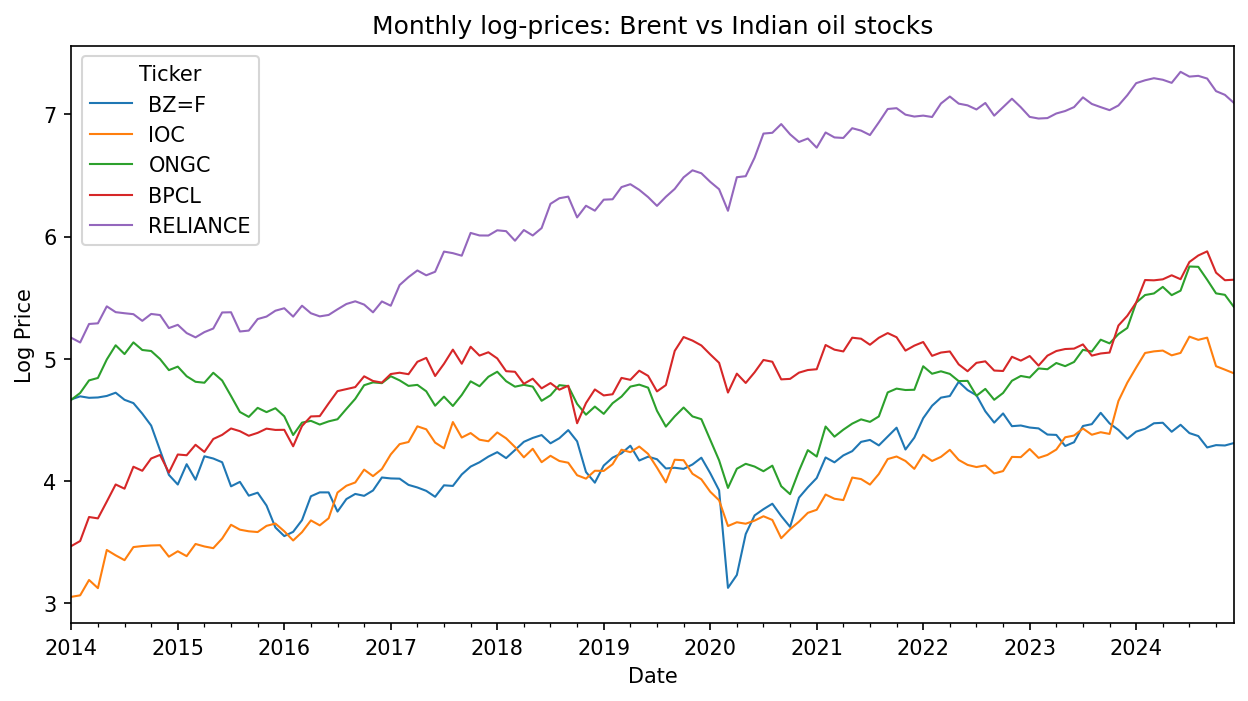
\includegraphics[width=0.9\textwidth]{prices_log_trend.png}
\caption{Monthly Log Prices: Brent Crude vs Indian Oil Stocks (2014--2024)}
\label{fig:prices}
\end{figure}

\begin{figure}[htbp]
\centering
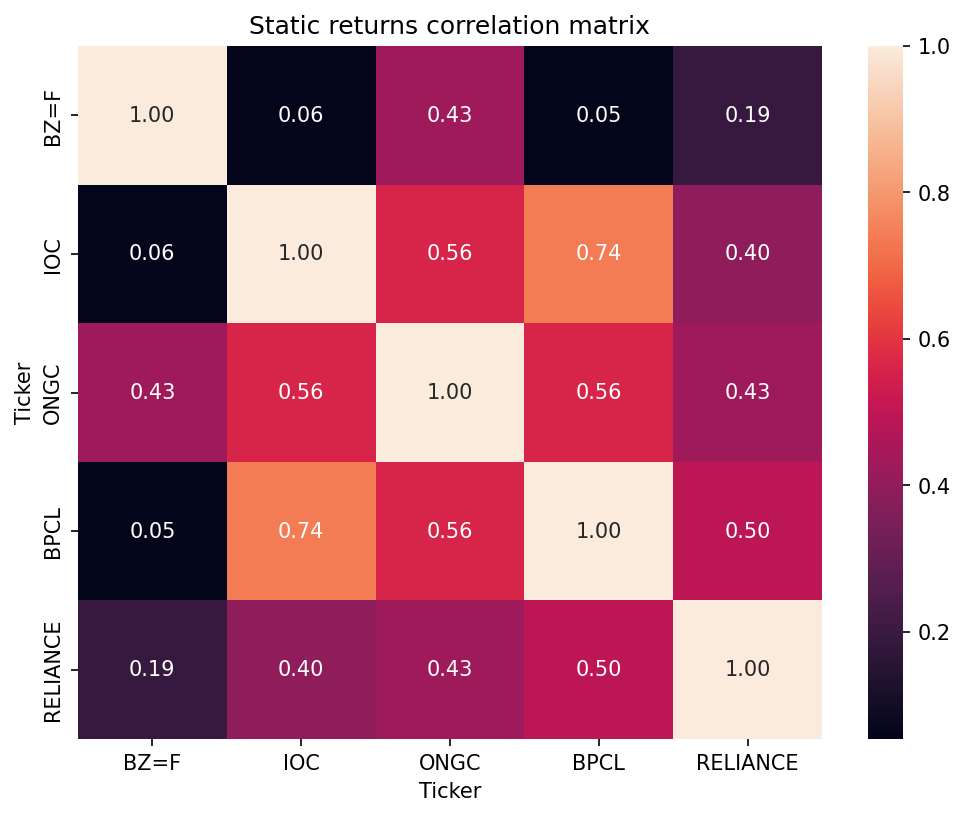
\includegraphics[width=0.85\textwidth]{corr_matrix.png}
\caption{Returns Correlation Matrix}
\label{fig:corr}
\end{figure}

\begin{figure}[htbp]
\centering
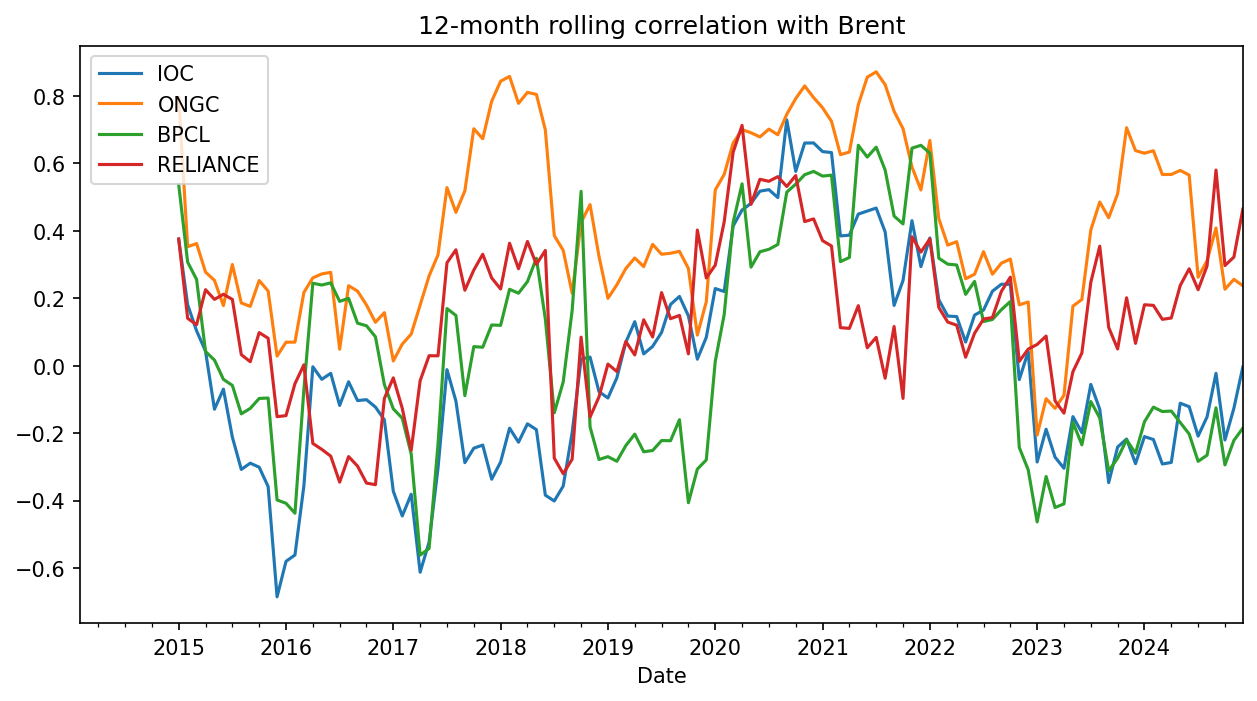
\includegraphics[width=0.9\textwidth]{rolling_corr_with_brent.png}
\caption{12-Month Rolling Correlation with Brent}
\label{fig:rolling_corr}
\end{figure}

\begin{figure}[htbp]
\centering
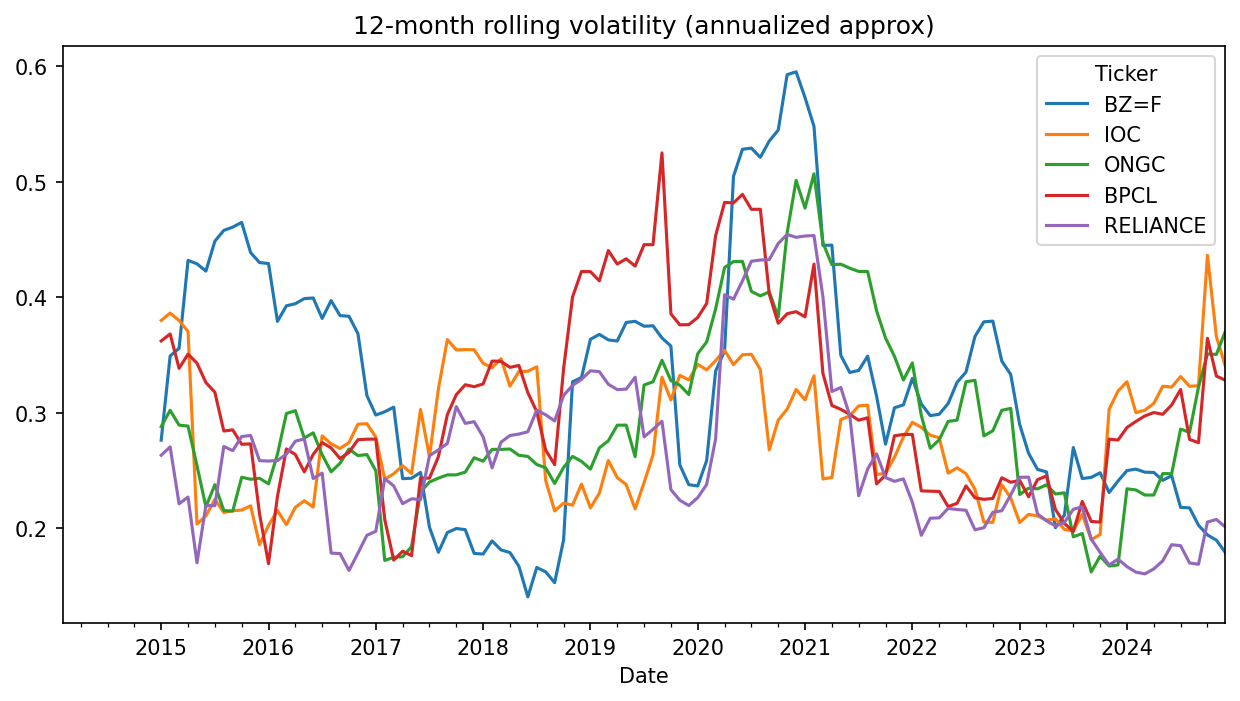
\includegraphics[width=0.9\textwidth]{rolling_volatility_12m.png}
\caption{12-Month Rolling Volatility (Annualized)}
\label{fig:rolling_vol}
\end{figure}

\begin{figure}[htbp]
\centering
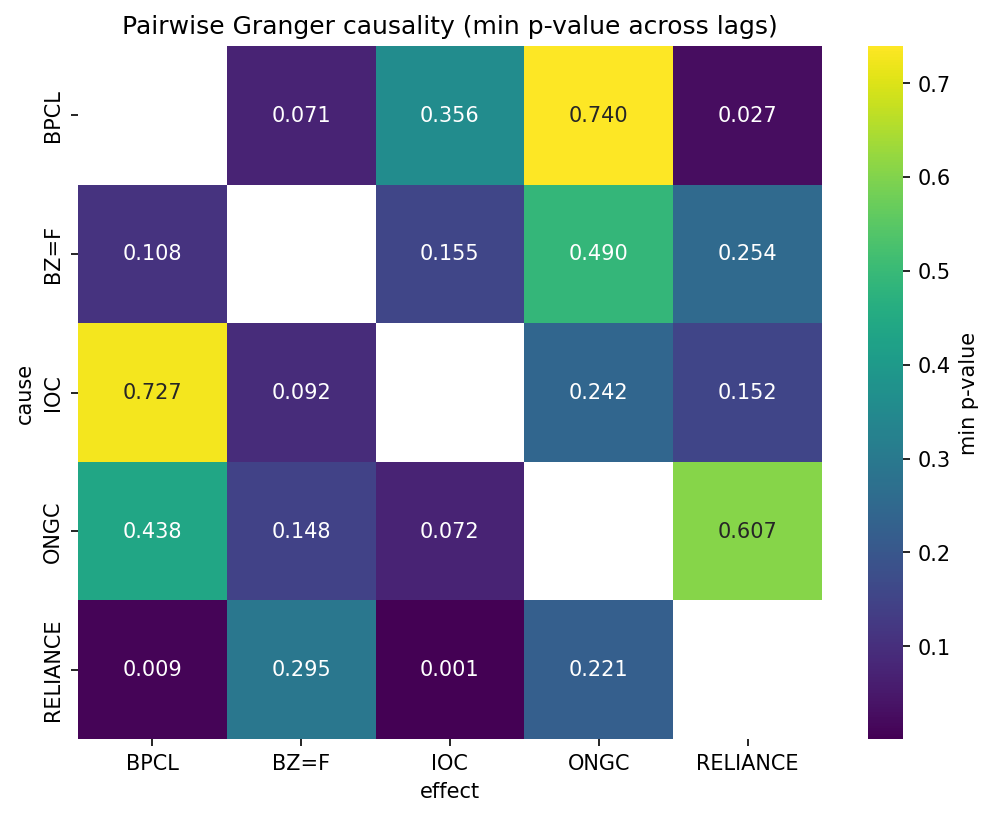
\includegraphics[width=0.85\textwidth]{granger_min_pvalues_heatmap.png}
\caption{Granger Causality Test Results (p-values)}
\label{fig:granger}
\end{figure}

\begin{figure}[htbp]
\centering
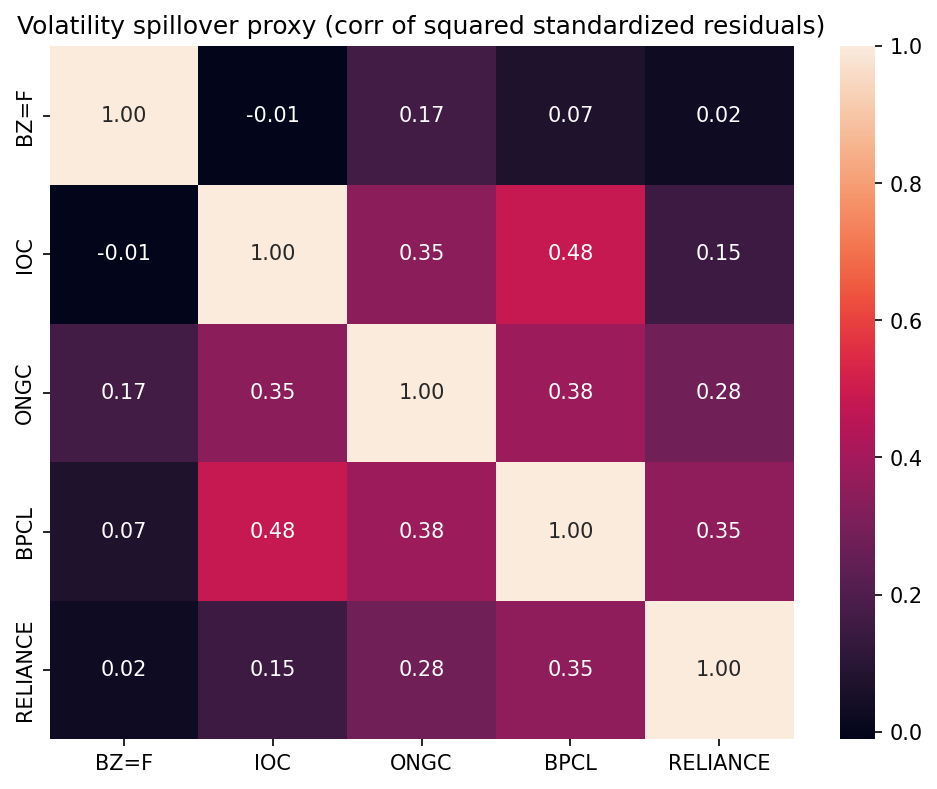
\includegraphics[width=0.85\textwidth]{volatility_spillover_heatmap.png}
\caption{Volatility Spillover Matrix}
\label{fig:vol_spillover}
\end{figure}

\begin{figure}[htbp]
\centering
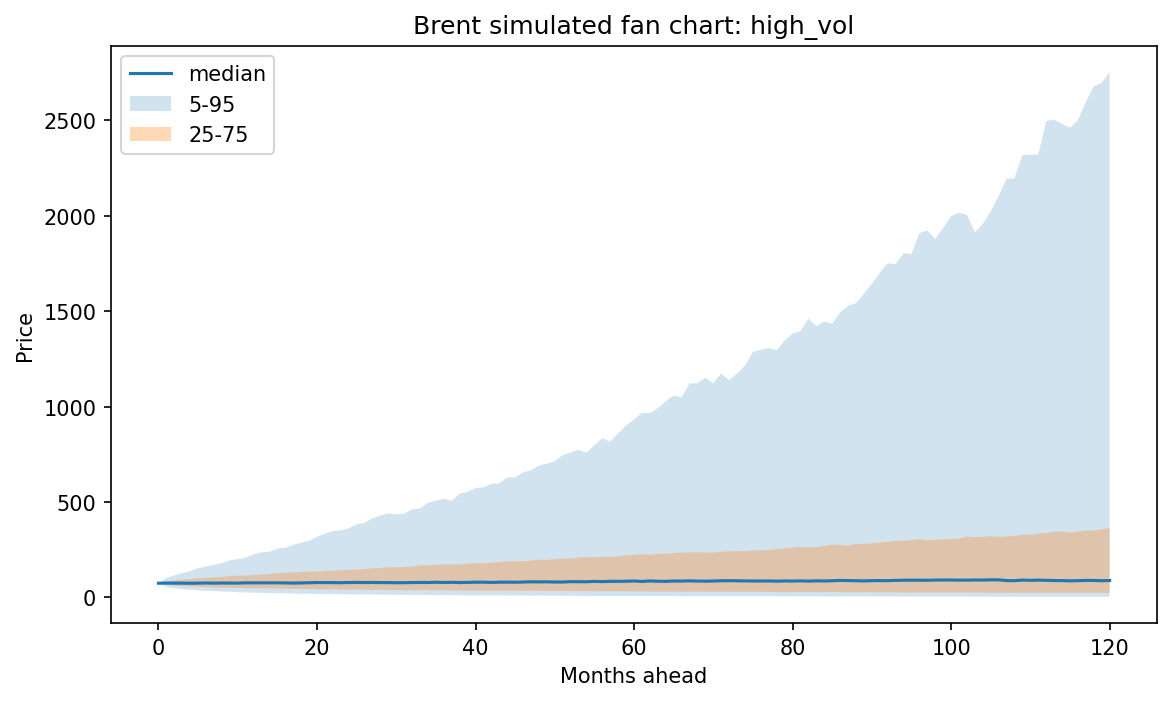
\includegraphics[width=0.9\textwidth]{fan_brent_high_vol.png}
\caption{Brent Crude Price Fan Chart: High Volatility Scenario (10-year projection)}
\label{fig:fan_brent}
\end{figure}

\begin{figure}[htbp]
\centering
\begin{subfigure}{0.48\textwidth}
    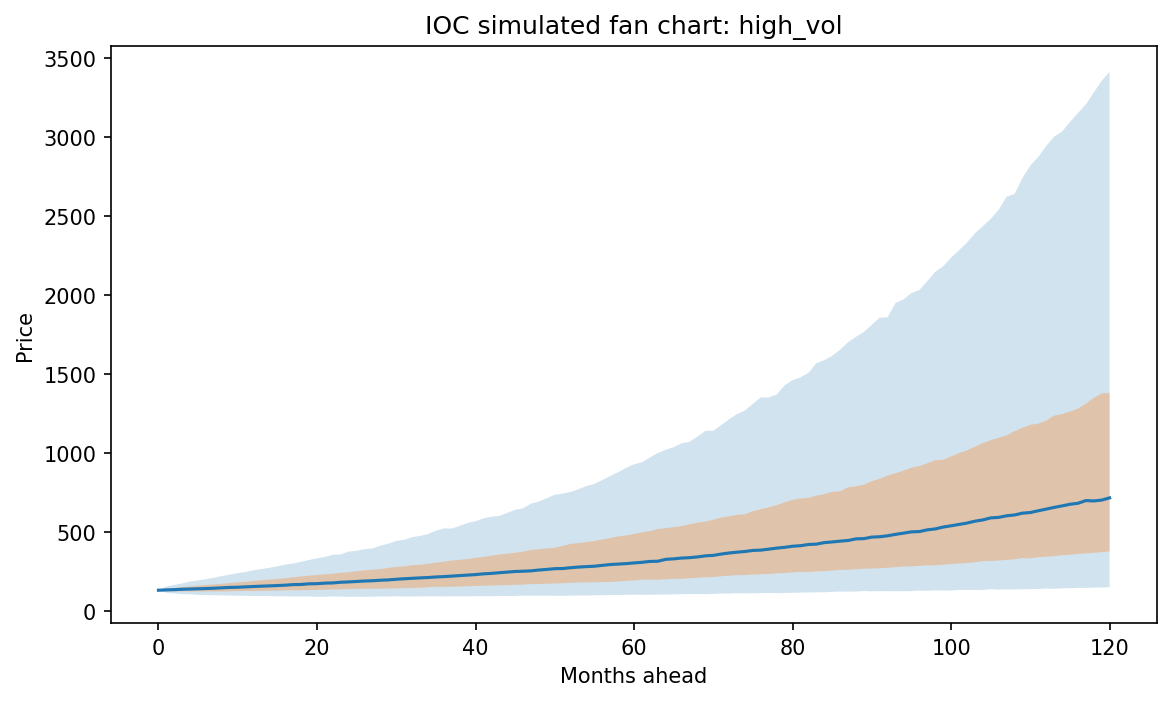
\includegraphics[width=\textwidth]{fan_IOC_high_vol.png}
    \caption{IOC}
\end{subfigure}
\hfill
\begin{subfigure}{0.48\textwidth}
    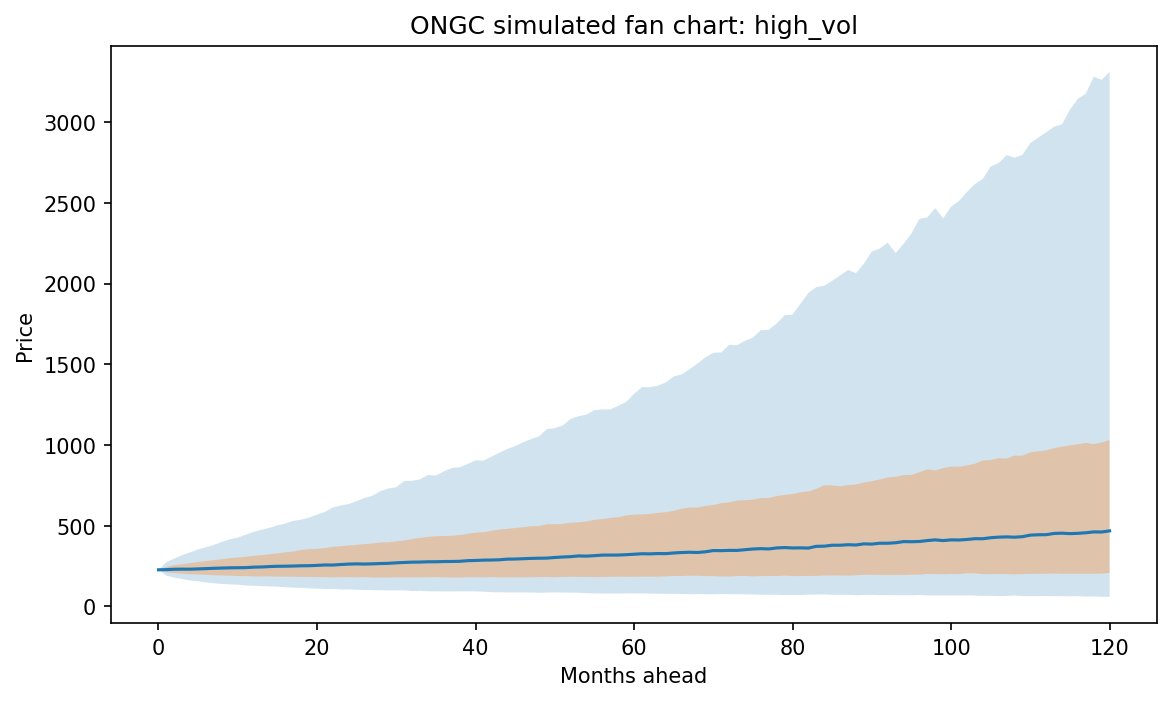
\includegraphics[width=\textwidth]{fan_ONGC_high_vol.png}
    \caption{ONGC}
\end{subfigure}

\vspace{0.5cm}

\begin{subfigure}{0.48\textwidth}
    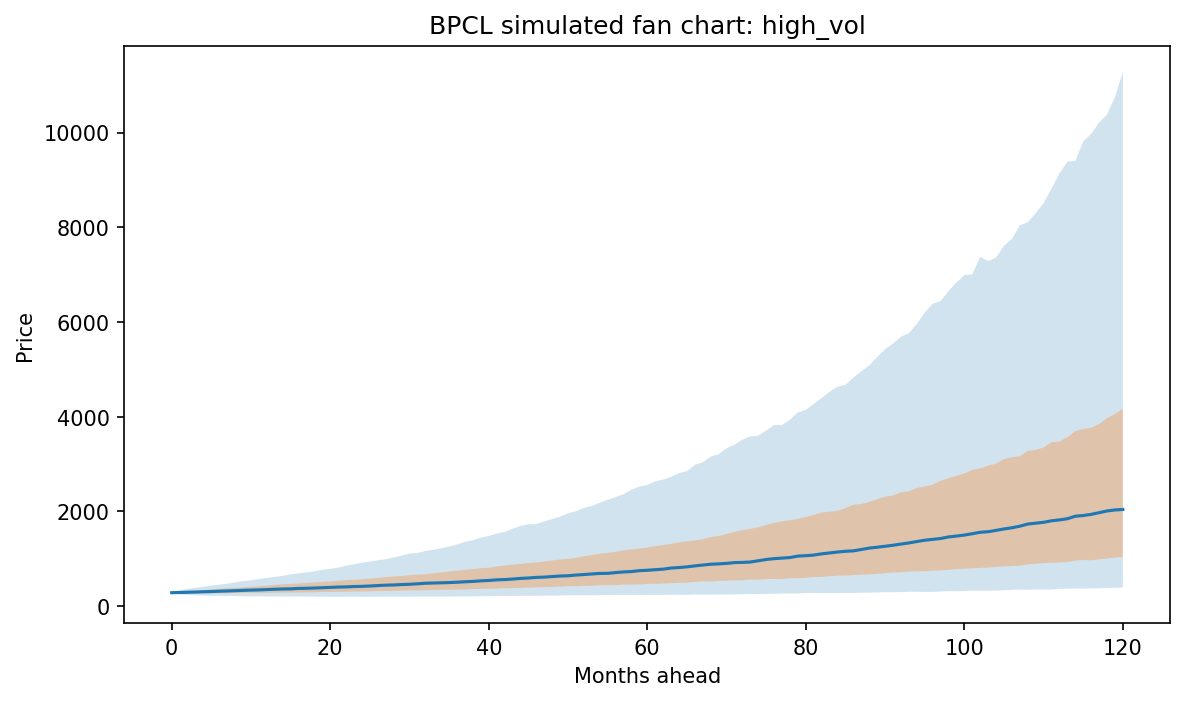
\includegraphics[width=\textwidth]{fan_BPCL_high_vol.png}
    \caption{BPCL}
\end{subfigure}
\hfill
\begin{subfigure}{0.48\textwidth}
    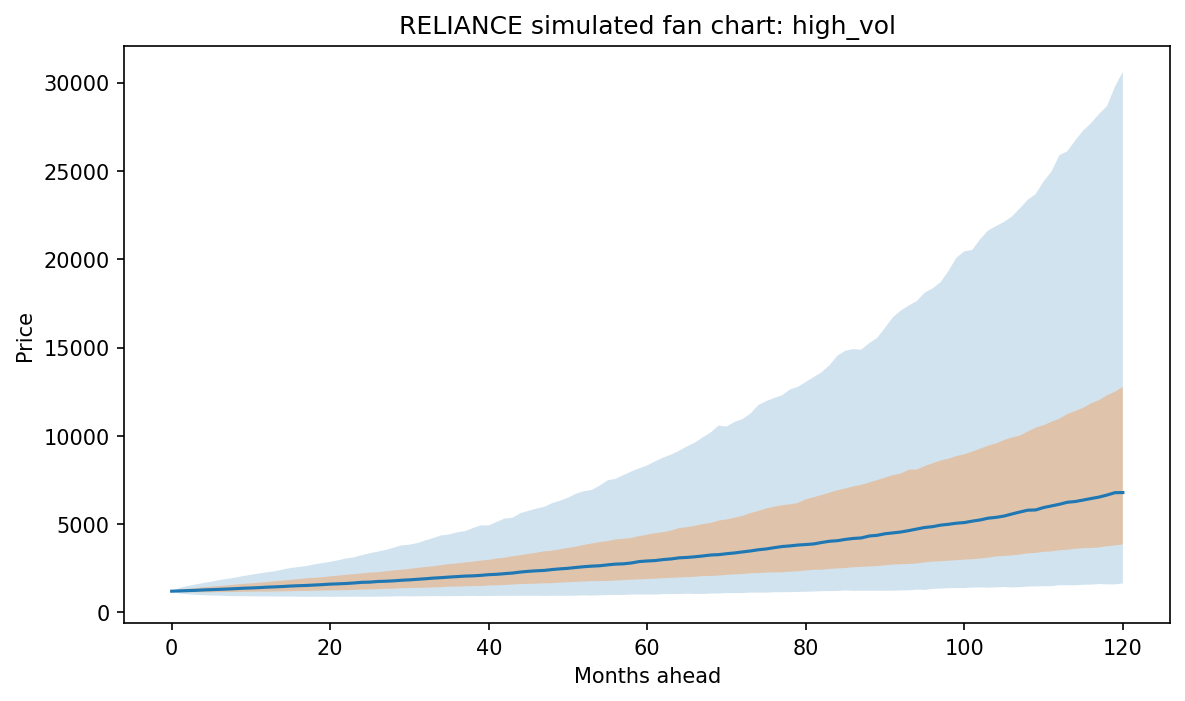
\includegraphics[width=\textwidth]{fan_RELIANCE_high_vol.png}
    \caption{RELIANCE}
\end{subfigure}

\caption{Indian Oil Stocks: 10-Year Price Projections (High Volatility Scenario)}
\label{fig:fan_stocks}
\end{figure}

% ===============================================
% KEY FINDINGS SECTION
% ===============================================
\clearpage
\section*{Key Findings}

\subsection*{1. Return Characteristics}
\begin{itemize}
    \item Monthly returns range from 0.14\% (Brent) to 1.66\% (BPCL)
    \item All series exhibit near-zero skewness except IOC (0.40) and RELIANCE (0.44)
    \item Kurtosis values suggest moderately heavy tails (0.02--1.08)
\end{itemize}

\subsection*{2. Correlation Structure}
\begin{itemize}
    \item ONGC shows strongest correlation with Brent (0.43***)
    \item Indian oil stocks highly correlated with each other (0.40--0.74***)
    \item IOC and BPCL exhibit highest inter-stock correlation (0.74***)
\end{itemize}

\subsection*{3. Time Series Properties}
\begin{itemize}
    \item All price series are non-stationary (unit root present)
    \item All return series are stationary (I(0) process confirmed)
    \item No cointegration detected among the five series (Johansen test)
    \item VAR(1) model appropriate for return dynamics
\end{itemize}

\subsection*{4. Market Linkages}
\begin{itemize}
    \item ONGC most sensitive to Brent movements ($\beta = 0.40$, $R^2 = 0.19$)
    \item RELIANCE shows moderate sensitivity ($\beta = 0.15$, $R^2 = 0.04$)
    \item IOC and BPCL exhibit minimal direct Brent exposure ($R^2 < 0.01$)
    \item Granger causality detected: IOC $\rightarrow$ RELIANCE, RELIANCE $\leftrightarrow$ BPCL
\end{itemize}

\subsection*{5. Volatility Dynamics}
\begin{itemize}
    \item Strong volatility persistence: GARCH $\beta$ coefficients 0.49--0.88
    \item IOC, ONGC, BPCL show highest persistence ($\beta > 0.83$)
    \item Moderate volatility spillovers among Indian stocks (0.15--0.48)
    \item Limited volatility transmission from Brent to Indian stocks
\end{itemize}

\subsection*{6. Common Factors}
\begin{itemize}
    \item First two PCs explain 78\% of return variation
    \item PC1 (53\%) represents broad market factor
    \item BPCL most exposed to PC1 ($\beta = 0.55$, $R^2 = 0.73$)
    \item Brent least explained by PC1 ($R^2 = 0.14$)
\end{itemize}

\subsection*{7. Scenario Projections (10-year, High Volatility)}
\begin{itemize}
    \item Brent median: \$88.60 (current: \$75), CAGR: 1.76\%
    \item BPCL shows highest growth potential: median ₹2,041 (CAGR: 21.83\%)
    \item Wide uncertainty bands reflect elevated volatility assumption
    \item 95th percentile outcomes suggest potential for extreme upside
\end{itemize}

\end{document}
